\chapter{Results and Discussion}\label{chapter5}

In this chapter we will demonstrate the results succeeded in proving the experiments were a success on the \dimsum task. Both the baseline and final systems provided solutions to the task while the Bi-LSTM-CRF outperformed the baseline.

The results section \ref{chapter5results} will mention the CRF baseline results and Bi-LSTM-CRF final results. Data splits will be briefly mentioned and can be read about in more details in the data section of the appendix \ref{appendixdata}. Epoch cutoffs are established and used for the final Bi-LSTM-CRF results and will be demonstrated. Final results for both systems will be compared.

The Discussion section will speak about comparisons of results with the original task publication, move on to the pitfalls of the design and finally discuss possible improvements for future work.

\section{Results}\label{chapter5results}
To ensure high quality results and remove ``contamination'' of testing data while training solutions, additional data splits were created from \dimsum task corpus. The data splits were used mainly for the Bi-LSTM-CRF but were nonetheless important in establishing a rigorous methodology for model training and comparisons. The \texttt{dimsum16.train} file was split into separate \texttt{train/dev/test} sets by percentages of \texttt{60/20/20} and \texttt{80/20/-} respectively. For more details on the data please refer to the appendix \ref{appendixdata}.

An example how evaluation is performed with additional images showing a misaligned prediction with supersense errors can be seen in Figure \ref{fig:linkmeasure} which was taken directly from the original \dimsum publication \cite{Schneider2016}.

\newcommand{\tagtss}[5]{\begin{tabular}{@{\hspace{2pt}}c@{\hspace{2pt}}} \texttt{#2\vphantom{\textlarger{Ĩ}}}\\ \sst{#3}\vphantom{X} \\ \textbf{#1}\vphantom{lp} \\ \sst{#5}\vphantom{X} \\ \texttt{#4\vphantom{\textlarger{Ĩ}}}\end{tabular}}
\newcommand{\sst}[1]{\textsc{#1}} % supersense category
\begin{figure}[H] %\small
% {``34'': [``price'', ``POSSESSION''], ``36'': [``means'', ``cognition''], ``26'': [``was'', ``stative''], ``29'': [``budge'', ``change'']}
\begin{framed}\small
\emph{MWE Precision:} The proportion of predicted links whose words 
both belong to the same expression in the gold standard. \\
\emph{MWE Recall:} Same as precision, but swapping the predicted and gold annotations. %\\
%\emph{Strength Averaging:} A weak link is treated as intermediate between a strong link and no link at all: 
%precision, recall, and $F_1$ computed on strong links only are averaged 
%with the respective calculations computed on all links without regard to strength.
\end{framed}\centering
\begin{tikzpicture}[baseline={($(current bounding box.center)+(0,-0.5ex)$)}, node distance=0cm, auto,]
 \node[inner sep=0cm]                                  (n1) {\tagtss{The}{O}{}{O}{}};
 \node[inner sep=0cm,above right=0pt of n1.south east] (n2) {\tagtss{staff}{O}{\textsc{n.group}}{\color{orange}B}{\color{orange}n.group}};
 \node[inner sep=0cm,above right=0pt of n2.south east] (n3) {\tagtss{leaves}{\color{red}B}{\color{red}v.cognition}{\color{orange}I}{}};
 \node[inner sep=0cm,above right=0pt of n3.south east] (n4) {\tagtss{a}{\color{blue}b}{}{\color{orange}I}{}};
 \node[inner sep=0cm,above right=0pt of n4.south east] (n5) {\tagtss{lot}{\color{blue}i}{}{\color{orange}I}{}};
 \node[inner sep=0cm,above right=0pt of n5.south east] (n6) {\tagtss{to}{\color{red}I}{}{\color{orange}I}{}};
%\path[-,thick,dotted, bend left=30] (n2.north) edge (n3.north); 
\path[-,thick,red, bend left=20] (n3.north) edge (n6.north);
 \path[-,thick,blue, bend left=30] (n4.north) edge (n5.north);
\path[-,thick,orange, bend right=20] (n2.south) edge (n3.south);
\path[-,thick,orange, bend right=20] (n3.south) edge (n4.south);
\path[-,thick,orange, bend right=20] (n4.south) edge (n5.south);
\path[-,thick,orange, bend right=20] (n5.south) edge (n6.south);
 \node[inner sep=0cm,above right=0pt of n6.south east] (n7) {\tagtss{be}{\color{red}I}{}{\color{orange}I}{}};
\path[-,thick,orange, bend right=20] (n6.south) edge (n7.south); 
 \node[inner sep=0cm,above right=0pt of n7.south east] (n8) {\tagtss{desired}{\color{red}I}{}{O}{v.emotion}};
\path[-,thick,red, bend left=30] (n6.north) edge (n7.north);
\path[-,thick,red, bend left=30] (n7.north) edge (n8.north);
 \node[inner sep=0cm,above right=0pt of n8.south east] (n9) {\tagtss{.}{O}{}{O}{}};
\end{tikzpicture}
\caption{A \textsc{Reviews} sentence with MWE and supersense analyses: gold above and hypothetical prediction below. 
MWE precision of the bottom annotation relative to the top one is $2/5$. %with weak links removed 
%and $2/6$ with weak links strengthened to strong links
(Note that a link between words $w_1$ and $w_2$ is ``matched'' 
if, in the other annotation, there is a path between $w_1$ and $w_2$.) 
The MWE recall value is $3/4$. 
Supersense precision and recall are both $1/2$.
Combined precision/recall scores add the respective subscores' numerators and denominators:
thus, combined precision is $\tfrac{2+1}{5+2} = 3/7$, 
and combined recall is $\tfrac{3+1}{4+2} = 2/3$.
Combined $F_1$ is their harmonic mean, i.e.~$12/23$.
%Overall $F_1$ is computed as the average of two $F_1$-scores, i.e.~$\tfrac{1}{3} \cdot \tfrac{1}{1}/(\tfrac{1}{3} + \tfrac{1}{1}) + \tfrac{2}{6}\cdot \tfrac{3}{3}/(\tfrac{2}{6}+\tfrac{3}{3}) = 0.50$.
}
\label{fig:linkmeasure}
\end{figure}

All final results are compared using F1-Scores from the \dimsum task's provided evaluation script \texttt{dimsumeval.py} to establish a framework for relational comparability. Additional results for precision, recall and accuracy will be presented for completeness.

\subsection{CRF Baselines}

Evaluation results are computed by using a combined mean of Recall, Precision, F1-Score and Accuracy for MWE and Supersense predictions. 

The combined score represents the averaged predictive results as seen in Figure \ref{fig:baselinescombinedresults}. For more verbose details on individual results please refer to the appendix \ref{appendixresults}.

\begin{figure}[H]
  \begin{minipage}{.5\textwidth}
    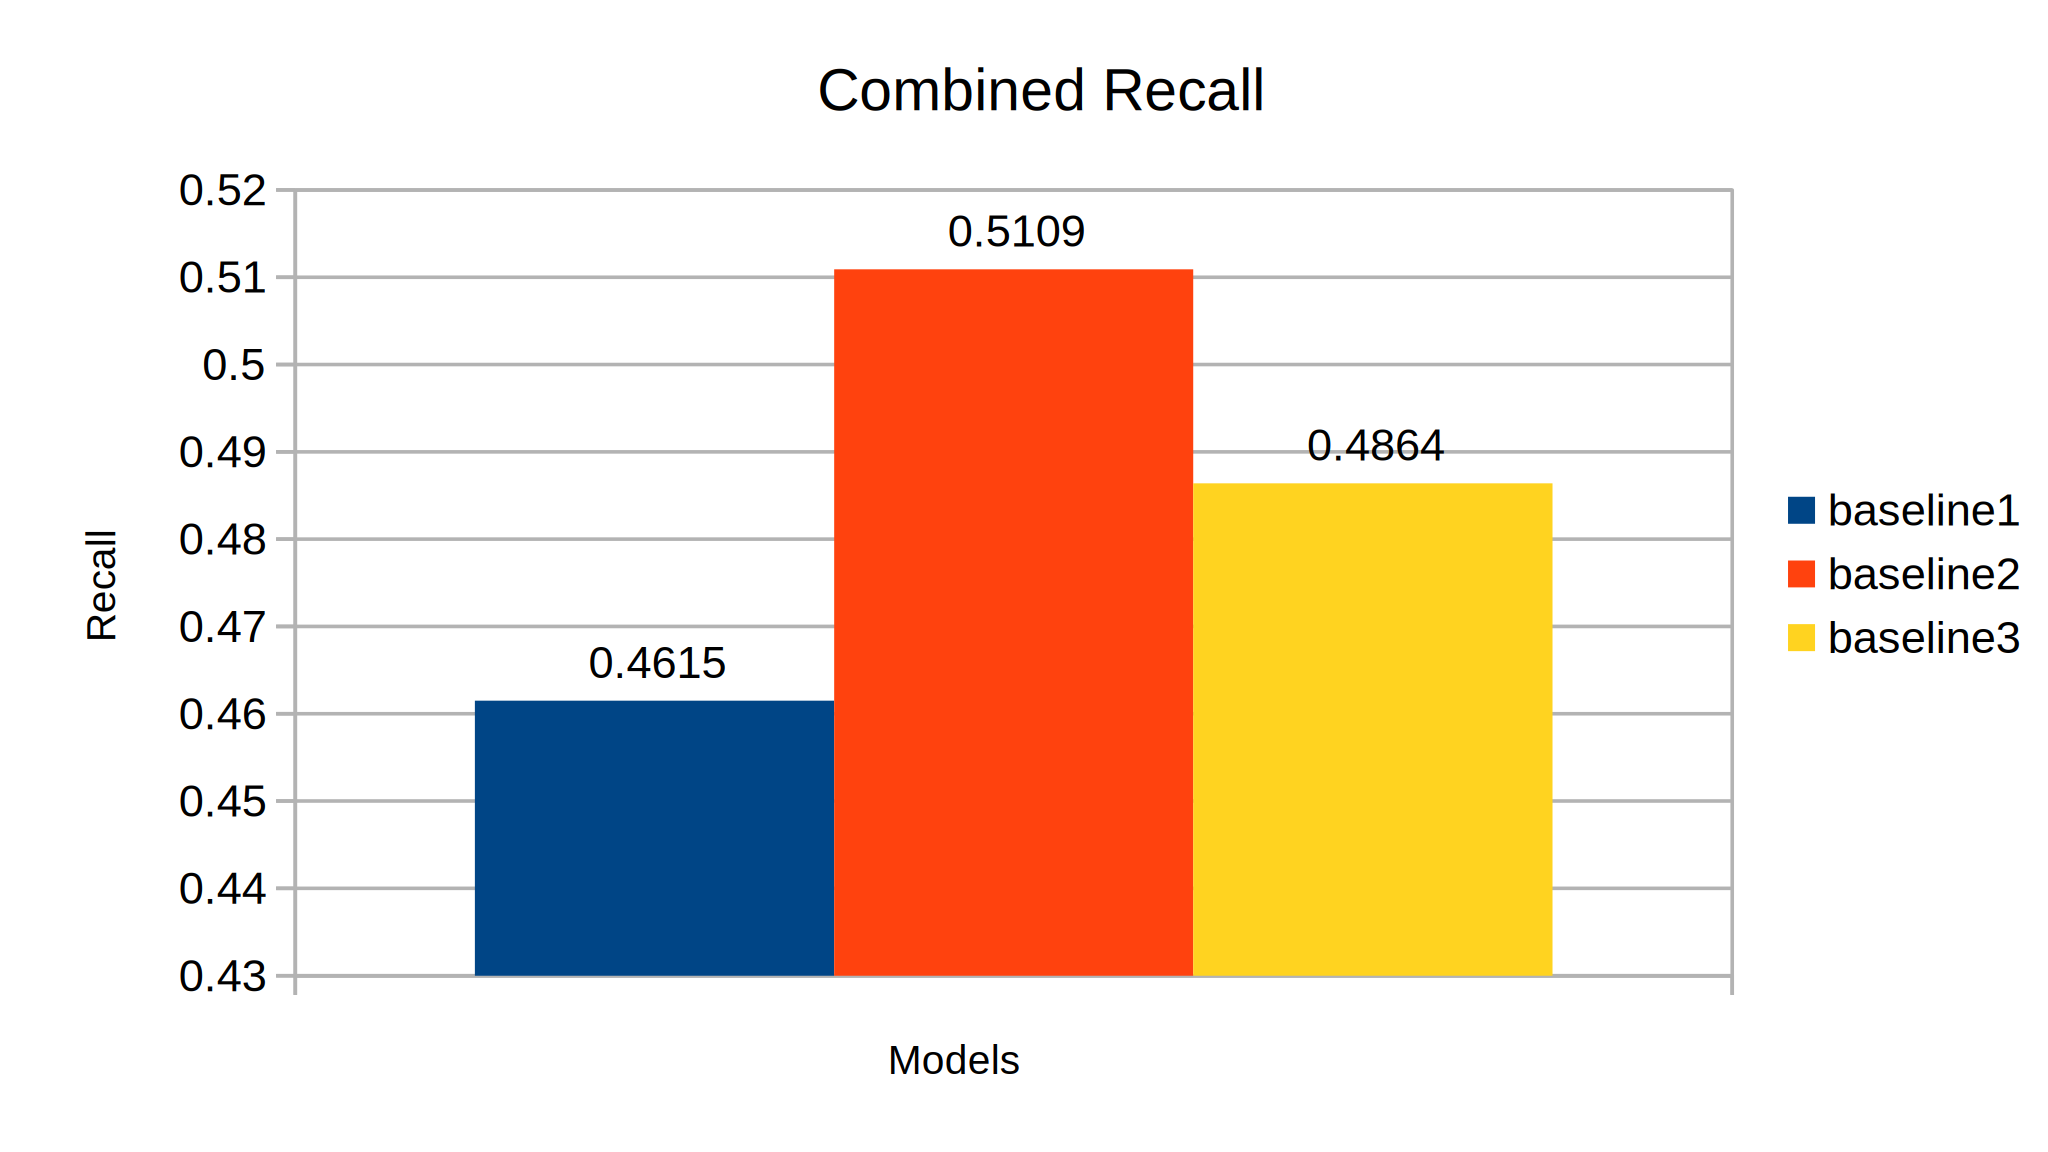
\includegraphics[width=\textwidth]{images/baselines_combined_recall.png}
    \centerline{Recall}\medskip
  \end{minipage}\hfill
  \begin{minipage}{.5\textwidth}
    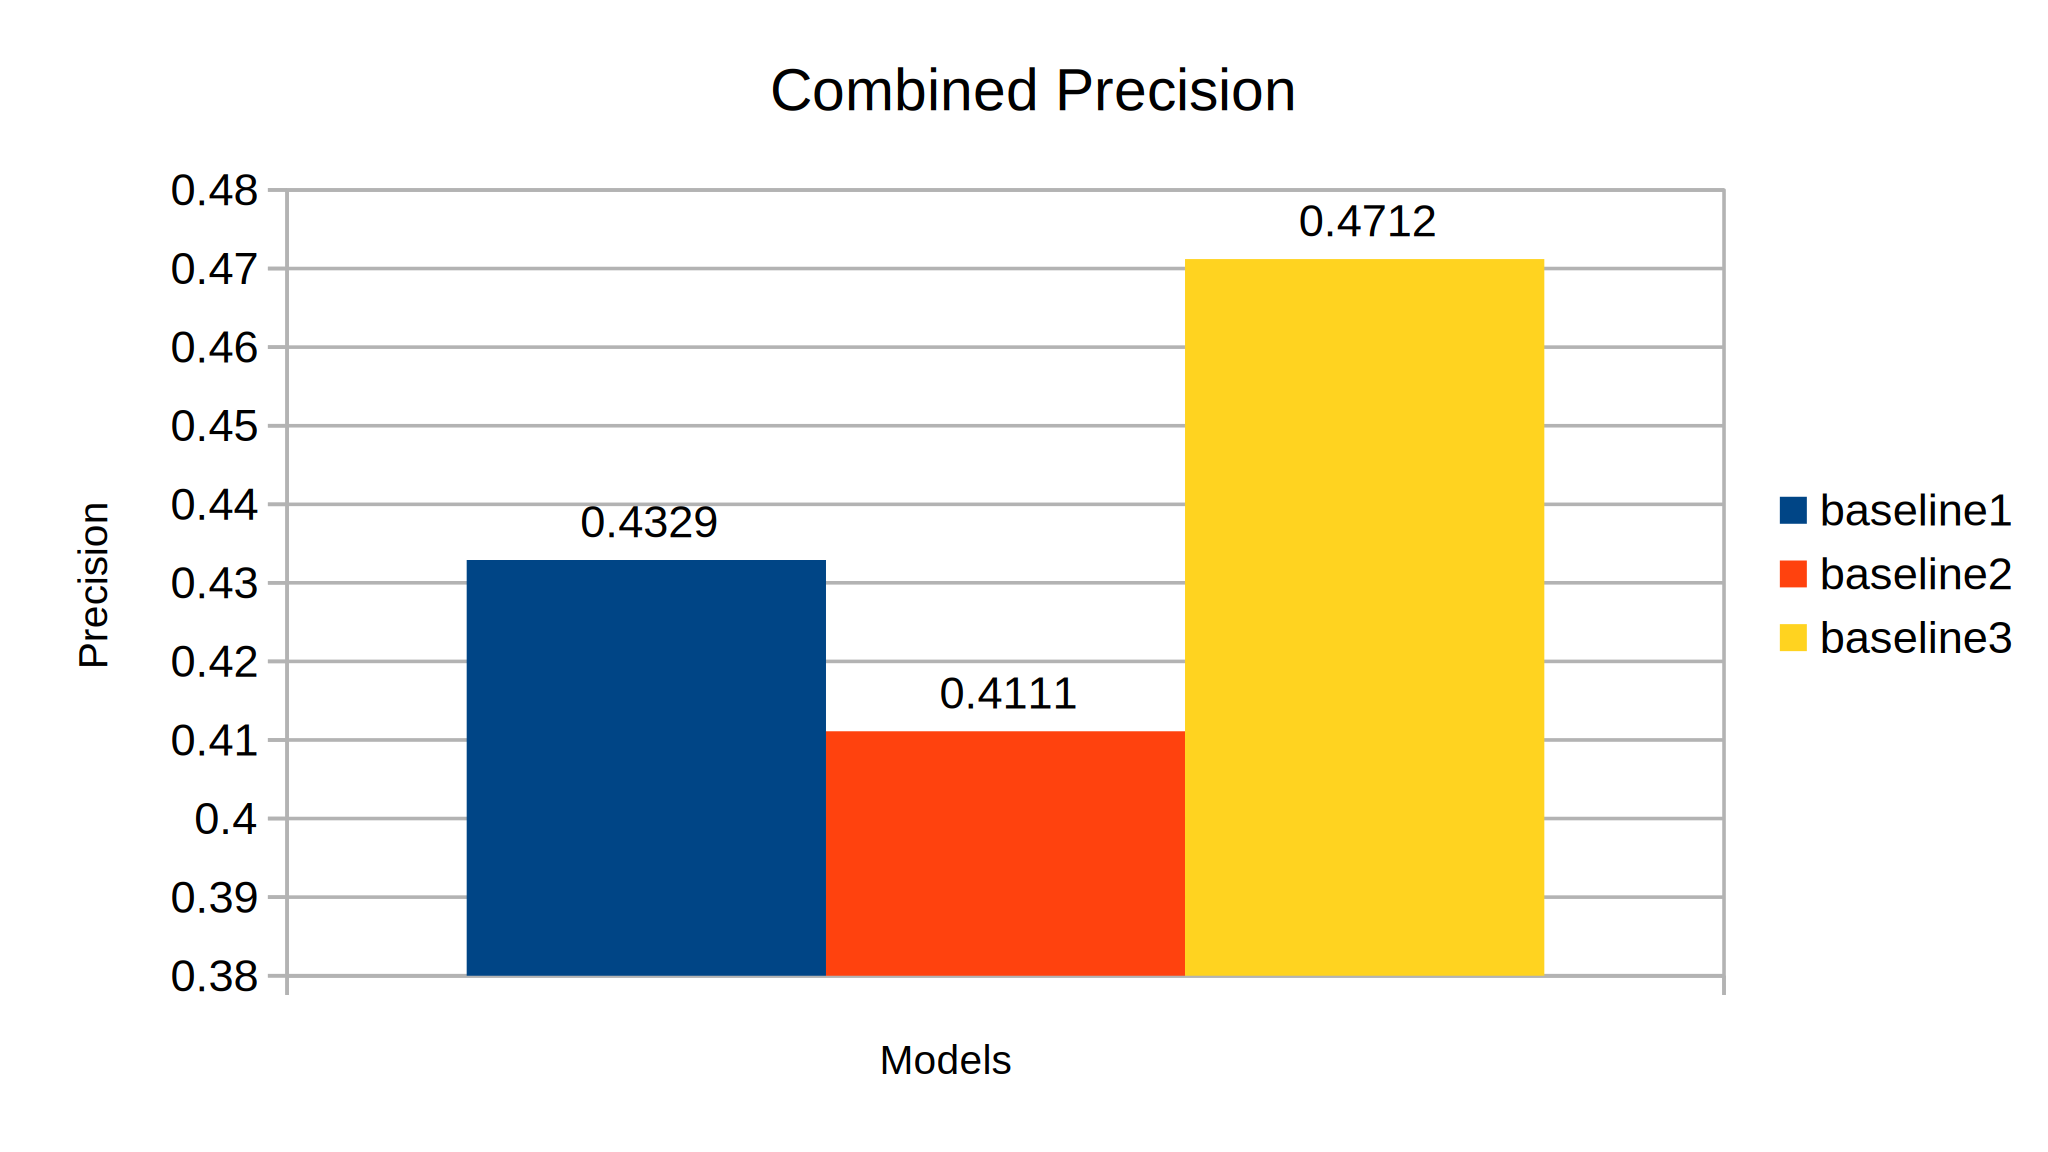
\includegraphics[width=\textwidth]{images/baselines_combined_precision.png}
    \centerline{Precision}\medskip
  \end{minipage}\\
  \begin{minipage}{.5\textwidth}
    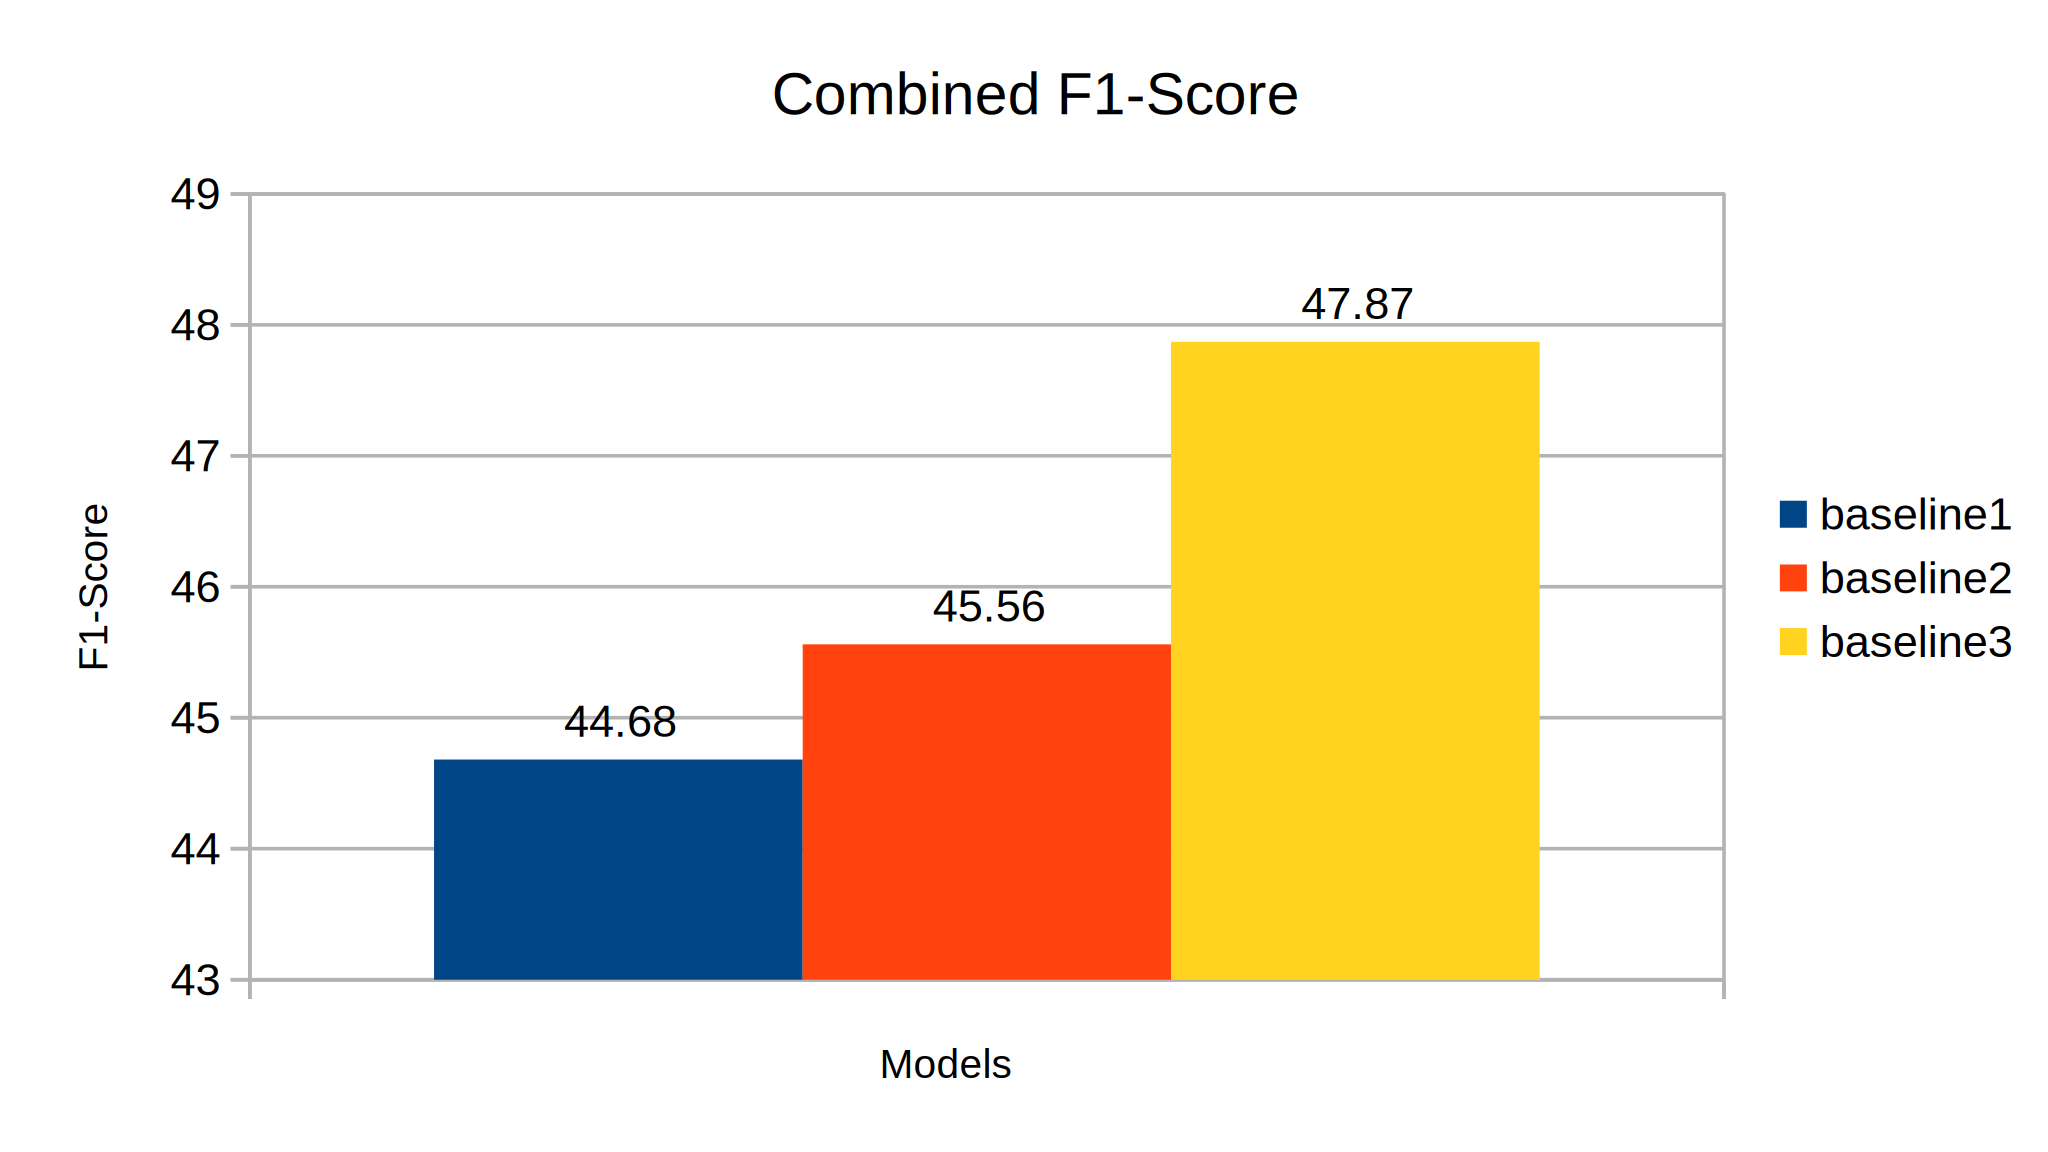
\includegraphics[width=\textwidth]{images/baselines_combined_f1score.png}
    \centerline{F1-Score}\medskip
  \end{minipage}\hfill
  \begin{minipage}{.5\textwidth}
    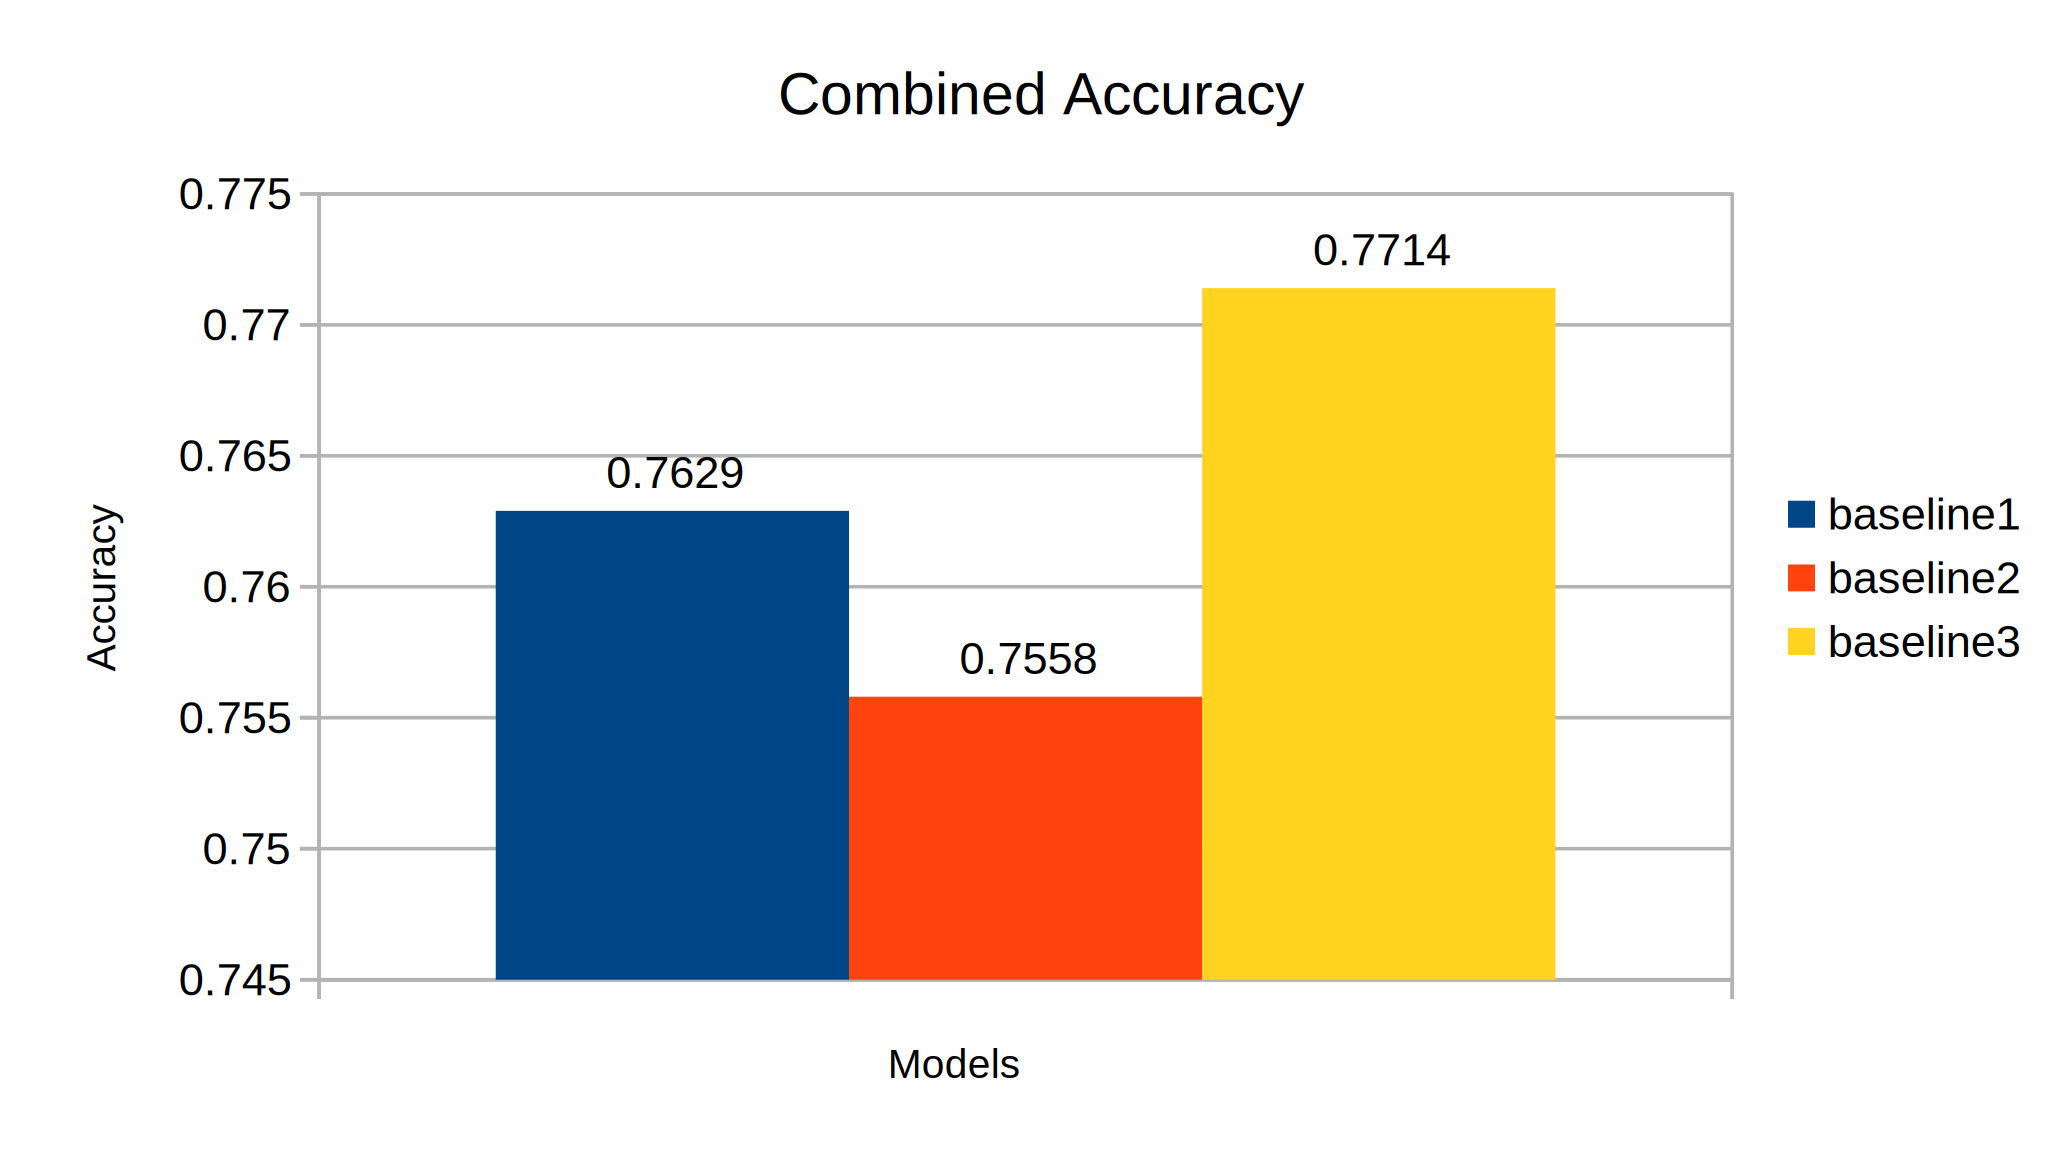
\includegraphics[width=\textwidth]{images/baselines_combined_accuracy.png}
    \centerline{Accuracy}\medskip
  \end{minipage}\\
  \begin{minipage}{\textwidth}
    \centerline{\includegraphics[width=0.7\textwidth]{images/baselines_combined_legend.png}}
  \end{minipage}
  \caption{Baselines Combined Results}
  \label{fig:baselinescombinedresults}
\end{figure}

The results for the baseline systems show that baseline number 3 produced a quantifiably higher result in all areas except Recall. The combined average F1-Score for baseline number 3 produced a 2.3\% increase over baseline 2 and 3.1\% increase over baseline 1. For this reason baseline number 3 was considered to be the best baseline for the \dimsum task. The characteristic difference was joint tags which directly lead to the correlation of ``jointness'' as the most influential aspect in performance.

\subsection{Bi-LSTM-CRF}
The use of the \texttt{60/20/20} data split from \texttt{dimsum16.train} was used for parameter optimisations to ensure complete separation from the \texttt{dimsum16.test} data, which was only used for the final results. 

During these initial tests, default parameters were used to determine epoch limitations. The default epoch limit was set to 100 but upon review of \texttt{dev} and \texttt{test} evaluations, over-fitting can be observed by around the 25th epoch as seen in Figure \ref{fig:bilstmcrfepochcutoff}. To save time for subsequent optimisation tests, a limit of 25 epochs was chosen for training. 

\begin{figure}[H]
\centering
\includegraphics[width=0.8\textwidth]{images/bi_lstm_crf_60_20_20_defaults_epoch_cutoff.png}
\caption{Bi-LSTM-CRF Epoch Cutoff}
\label{fig:bilstmcrfepochcutoff}
\end{figure}

Over 100 separate tests were done in order to optimise parameters for training on the \dimsum data \footnote{Appendix \ref{appendixresults} contains full table of training model results}. Training the optimised models took around 2 to 4 hours to complete on the university's computing cluster \texttt{iceberg}.

The final results using the \texttt{80/20/-} split with \texttt{dimsum16.test.blind} can be seen in Figure \ref{fig:bilstmcrfresults} where the leftmost line graph displays an average of F1-Score's over epochs and the rightmost bar graph shows the MWE, Supersense and Combined F1-Scores for the final trained model. 
\begin{figure}[H]
  \begin{minipage}{.5\textwidth}
    \includegraphics[width=\textwidth]{images/bi_lstm_crf_80_20_final_epochs_line_graph.png}
    \centerline{\footnotesize Training epochs F1-Scores}\medskip
  \end{minipage}\hfill
  \begin{minipage}{.5\textwidth}
    \includegraphics[width=\textwidth]{images/bi_lstm_crf_80_20_final_f1scores_bar_graph.png}
    \centerline{\footnotesize Testing MWE, Supersense and Combined F1-Scores}\medskip
  \end{minipage}\\
  \caption{Bi-LSTM-CRF Results}
  \label{fig:bilstmcrfresults}
\end{figure}

As demonstrated graphically, the final results are a combined F1-Score of 53.27\% which is a 5.4\% increase over the highest scoring baseline. Additional details about contributing factors to results will be mentioned in the discussion section \ref{chapter5discussion}.

\subsection{Comparisons}\label{chapter5resultscomparisons}
A comparison of results obtained from evaluations of CRF baselines, Bi-LSTM-CRF and published results from \cite{Schneider2016} will be presented in this section.

The original publication used team names and system numbers prefixed with ``\texttt{S}'' to distinguish solution submissions for the \dimsum task. In the table below, all results are shown from the original publication compared to the CRF Baseline systems and the final Bi-LSTM-CRF evaluation results. 
\begin{figure}[H]
  \begin{minipage}{\textwidth}
    \centering
    \begin{tabular}{|l|l|l|l|}
      \hline
      \textbf{System} & \textbf{Team}  & \textbf{Score} & \textbf{Resources}\\
      \hline
      \hline
      \texttt{S214} & ICL-HD & 57.77 & ++ \\
      \hline
      \texttt{S249} & UW-CSE & 57.71 & ++ \\
      \hline
      \texttt{S248} & UW-CSE & 57.10 &    \\
      \hline
      \texttt{\it Bi-LSTM-CRF} & & \hl{\bf 53.27} & ++ \\
      \hline
      \texttt{S106} & UFRGS\&LIF & 50.27 &   \\
      \hline
      \texttt{S227} & VectorWeavers & 49.94 & ++ \\
      \hline
      \texttt{\it CRF Baseline 3} & &  47.87 &   \\
      \hline
      \texttt{S255} & UTU & 47.13 & ++ \\
      \hline
      \texttt{S211} & UTU & 46.17 & + \\
      \hline
      \texttt{S254} & UTU & 45.79 &   \\
      \hline
      \texttt{\it CRF Baseline 2} & & 45.56 &   \\
      \hline
      \texttt{\it CRF Baseline 1} & & 44.68 &   \\
      \hline
      \texttt{S108} & WHUNlp & 25.71 &   \\
      \hline
    \end{tabular}
  \end{minipage}\\
  \begin{minipage}{\textwidth}
    \includegraphics[width=\textwidth]{images/systems_comparison_bar_graph.png}
  \end{minipage}
  \caption{System F1-Scores Comparison}
  \label{fig:systemsf1scorescomparison}
\end{figure}

The team name for the results is the author's name shown in italics while the highest scoring solution created for this dissertation is highlighted and printed in bold. All data is provided from highest scoring systems to lowest. 

In addition, Figure \ref{fig:systemsf1scorescomparison} shows a bar graph to demonstrate the data in an alternative manner with the four systems created for this dissertation coloured in while the original publication's results are shown in black and white with varying hatch marks only. 

The plus symbols are used to describe the data condition types (as mentioned in Chapter \ref{chapter3}) which are ``supervised closed'', ``semi-supervised closed'' and ``open''\footnote{As stated in \cite{Schneider2016}, ``The final column indicates the resource condition: systems entered in the open condition (all resources allowed) are designated “++”; “+” indicates the more restricted semi-supervised closed condition, while the remaining systems are in the closed condition (most restrictive).''}. The baseline systems used the most restrictive condition of supervised closed, using only the data provided for the original \dimsum task. Due to the usage of the pre-computed word embeddings, the final Bi-LSTM-CRF is considered to be in the least restrictive data condition category of ``open''.

\section{Discussion}\label{chapter5discussion}
A reflection of system capabilities is paramount to understanding quantifiable scientific findings after an evaluation has been performed. Self-examination and critique allows for further work to be developed and possible additions to be made to increase performance. This section intends to speak about intrinsic evaluation findings and potential pitfalls of the systems developed. By making such a critique, improvements will be considered for future enhancements and adaptions.  

For the most part, the discussion will be focused on the final result using the Bi-LSTM-CRF. The observations, pitfalls and improvements will cover the final model's approach to the \dimsum task.

\subsection{Intrinsic observations}
Some observations during the Bi-LSTM-CRF optimisation are notable for different reasons, but are mainly considered important for future developments using a similar model. A couple interesting points will be presented here. 

\subsubsection{CRF Layer}

The final layer of the Bi-LSTM-CRF as seen in Figure \ref{fig:lstmcrfexampledimsumdata} shows a final output CRF layer. This layer can be disabled in the adapted code, and during the optimisation process it was one of the tests that was performed. The joint tag predictions were based only on the combined Bi-LSTM output. As seen in Figure \ref{fig:602020crflayerenabledisablelinegraph}, a clear difference between the usage of the CRF layer to encode contextual information can be seen to be beneficial. The upper most lines show the CRF layer enabled and the bottom most lines show the CRF layer disabled demonstrated by using the plus and minus symbols for enabled and disabled respectively. The tests were done using the \texttt{60/20/20} data split from \texttt{dimsum16.train}. The first few epochs when disabling the CRF layer has some missing data points due to precision or recall being zero which lead to 'nan' values for F1-Scores.

\begin{figure}[H]
  \includegraphics[width=\textwidth]{images/bi_lstm_crf_60_20_20_crf_comparison_training_line_graph.png}
  \caption{60/20/20 Training epochs for CRF Layer Enabled/Disabled}
  \label{fig:602020crflayerenabledisablelinegraph}
\end{figure}

The difference between disabling and enabling the CRF layer is about 24 to 28 percent for test and dev respectively using the \texttt{60/20/20} split during training. By disabling the CRF layer in the code, you remove the additional power of the CRF which uses transitions and observation compiled by the training data to determine the most likely joint tag candidate. 

Training and testing with the \texttt{80/20/-} split and testing with the \texttt{dimsum16.test.blind} shows similar results as seen in Figure \ref{fig:8020crflayerenabledisablebargraph} with a difference of 21\% between disabling and enabling the CRF Layer.

\begin{figure}[H]
  \includegraphics[width=\textwidth]{images/bi_lstm_crf_80_20_crf_comparison_test_bar_graph.png}
  \caption{80/20 Test results for CRF Layer Enabled/Disabled}
  \label{fig:8020crflayerenabledisablebargraph}
\end{figure}

The use of the CRF in both models cannot be directly correlated as the features are not comparable. That being said, it can be argued that using the Bi-LSTM without the CRF layer for the \dimsum task cannot outperform a simple single CRF solution for joint tag prediction as seen in CRF baseline 3. An alternative configuration with different Bidirectional features may prove otherwise, but in it's current configuration the CRF layer is a valuable addition to the model even though it's true importance, either temporal or other, is not known. 

\subsubsection{Pre-embeddings}

The single most important optimisation to the model was using pre-embeddings. As seen in Figure \ref{fig:preembcomparison}, the performance gain jumped from 44.31\% to 53.27\% providing a 8.96\% increase over the same optimised model without pre-embeddings\footnote{Initial few epochs without pre-embeddings provided \texttt{nan} F1-Scores}.

\begin{figure}[H]
  \begin{minipage}{.5\textwidth}
    \includegraphics[width=\textwidth]{images/bi_lstm_crf_80_20_preembeddings_comparison_line_graph.png}
    \centerline{\footnotesize Training epochs F1-Scores}\medskip
  \end{minipage}\hfill
  \begin{minipage}{.5\textwidth}
    \includegraphics[width=\textwidth]{images/bi_lstm_crf_80_20_preembeddings_comparison_bar_graph.png}
    \centerline{\footnotesize Testing Combined F1-Scores}\medskip
  \end{minipage}\\
  \caption{Pre-embeddings comparison}
  \label{fig:preembcomparison}
\end{figure}

Most likely the pre-computed word embeddings provided much richer contextual detail to the input word vectors which was the key factor in boosting performance. These findings seem to be in line with other observations as seen in \cite{Schneider2016}.

\subsection{Pitfalls}\label{chapter5discussionpitfalls}

Critiquing the systems and data design can help determine failures in models and assumptions about data. This section intends to speak about both with specific attention to data usage.

\subsubsection{Joint tags as Predictive labels}
The final Bi-LSTM-CRF system uses labels read from training data. There are benefits and issues for this model. 

Using joint tags eliminated issues in prediction where {\bf B}eginning MWE tags were not coupled with supersenses, as all potential combinations in the training data inherently followed the structural limitation of MWE \texttt{[B|b]} and supersense tag coupling.

Every system designed has instances in which the MWE tags \texttt{{BbIiOo}}, were predicted in an invalid way, e.g. a sequence of only \texttt{I} labels without a \texttt{B}. In the majority of cases the {\bf B}eginning tags \texttt{[B|b]} were predicted in a wrong location or not predicted at all. This would mean that in a joint tag system, the only potential limitation would be failures in MWE tag prediction. Issues in regards to MWE tag prediction are spoken of more in the following section \ref{pitfallsmwes}.

The final Bi-LSTM-CRF model used, determines possible labels during training by reading data only, and not using a predefined set. One issue involved in using joint tags as predictive labels in the current configuration is that not all joint tags can be known from the training data. 

There are 6 possible tags for MWE tag sequences and 41 possible tags for Supersenses\footnote{the WordNet Supersense \texttt{n.Tops} is not used, otherwise there would be 42 possible Supersenses.} as seen in Section \ref{tab:wordnetsupersenses}. The cross product would give us a quantity of 246 possible tags. 

\begin{align*}
   |\{BbIiOo\}| \times |\{Supersenses\}| = 246
\end{align*}

In the \texttt{dimsum16.train} file only 118 joint tags can be constructed from reading the data alone. This means only 47\% of the possible joint tag labels are represented as seen in Table \ref{tab:jointtagcountsrepresented}.

\begin{table}[H]
    \centering
    \begin{tabular}{l|l|l}
      Cross-product Maximum & 246 & {\bf Total represented}\\
      \hline
      dimsum16.train & 118 & 47.07\%\\ 
      dimsum16.test & 90 & 36.59\%\\ 
    \end{tabular}
  \caption{Joint tag label counts with percent represented in data}
  \label{tab:jointtagcountsrepresented}
\end{table}

The benefit of creating a predictive label set from training data is flexibility, and that the system can work with minimal alterations for new labels. The downside is all of the unseen labels are mapped to the most frequent label, in our case the {\bf O}utside tag with no supersense.  

In our test data there are 90 joint tags and only 3 are not seen in the training data. Each of the 3 joint tag labels is seen only once. Therefore by predicting the highest probable joint tag label of ``\texttt{O\_\_}'' we introduce a negligible error. It these default labels introduced a complete MWE tag sequence error, it could only possibly decrease accuracy for MWE tag sequences by a maximum of 0.3\%.

All this being said, to make a more robust system, there should be a better way for handling unknown labels, such as giving the system the full set of possible labels beforehand. 

\subsubsection{MWEs}\label{pitfallsmwes}

The quantity of MWE tag sequences found to be invalid were only 16 in CRF Baseline 3 and 21 in the optimised Bi-LSTM-CRF. There were only 1000 test sentences so there was a total of 1.6\% to 2.10\% invalid MWE sequence predictions for CRF Baseline 3 and the optimised Bi-LSTM-CRF respectively. This can obviously be improved but shows that ``patching'' invalid sequences with \texttt{O} tag sequences can only introduce a 1.6-2.1\% error.

Interestingly enough, the valid sequences of sequential {\bf O}utside tags were about 14\% to 18\% of the MWE tag sequences that were predicted incorrectly as seen in Table \ref{tab:inseqoutmwetagseq}. 

\begin{table}[H]
    \centering
    \begin{tabular}{ll}
      Baseline 3 & Bi-LSTM-CRF\\
      \hline
      146 / 1000 & 186 / 1000\\
      14.6\% & 18.6\%
    \end{tabular}
  \caption{Incorrect Sequential {\bf O}utside MWE tag sequence}
  \label{tab:inseqoutmwetagseq}
\end{table}

This means that up to 18\% of incorrect MWE tag sequences had no MWEs predicted when they should have been. 

In a strictly accuracy based sense for entire MWE tag sequences, without regard to alignment or quantity of MWEs, there are a total of 480 and 492 invalid MWE tag sequences as seen in Table \ref{tab:accuracyinvalidtagseq}. 

\begin{table}[H]
    \centering
    \begin{tabular}{ll}
      Baseline 3 & Bi-LSTM-CRF\\
      \hline
      480 / 1000 & 492 / 1000\\
      48.0\% & 49.2\%
    \end{tabular}
  \caption{Accuracy of Invalid MWE tag sequences}
  \label{tab:accuracyinvalidtagseq}
\end{table}

This means that about 30\% to 37\% of all inequivalent MWE tag sequences to the gold test data were due to the fact that no MWE was predicted when there should have been at least one. 

Figure \ref{fig:nomwepred} shows how all outside tags were predicted when there is in fact a single MWE with a length of 2.

\begin{figure}[H]
    \centering
    \begin{tabular}{l|lllllllll}
           & So & what & was & the & point & of & the & appointment & !?!\\
      \hline
      \rowcolor{yellow!50}
      GOLD & O  & O    & O   & B   & I     & O  & O   & O           & O\\
      PRED & O  & O    & O   & O   & O     & O  & O   & O           & O\\
    \end{tabular}
  \caption{Example of no MWE tags predicted}
  \label{fig:nomwepred}
\end{figure}

For the remaining 334 and 306 sentences, MWEs were not predicted correctly. This could be due to misalignment, length inconsistencies or incorrect quantities of MWEs predicted in each sentence. As seen in table \ref{tab:mwetagseqinacccounts}, the majority of MWEs predicted on a per sentence basis were ``insufficient'' meaning, not enough MWEs were predicted, about 1/5 of the time. 

\begin{table}[H]
    \centering
    \begin{tabular}{l|l|l}
      & Baseline 3 & Bi-LSTM-CRF\\
      \hline
      Excessive & 9.17\% & 8.54\%\\
      Insufficient & 21.25\% & 20.12\%\\
    \end{tabular}
  \caption{MWE Quantity inaccuracy counts in sentences}
  \label{tab:mwetagseqinacccounts}
\end{table}

Finally, the residual amount of MWEs can only be either misaligned or have length inconsistencies. As seen in Figure \ref{tab:mwelengthalignmentinconsistencies} the issue is just about split down the center meaning that length and alignment issues are equally important for MWE sequences that have the correct quantities of MWEs. Described in an alternative manner; sentences which have the same amount of MWEs and have MWE tag sequence prediction errors are equally likely to be either misaligned or be the wrong length.

\begin{table}[H]
    \centering
    \begin{tabular}{l|l|l}
      & Baseline 3 & Bi-LSTM-CRF\\
      \hline
      Wrong Length & 49.7\% & 46.7\%\\
      Misaligned & 49.1\% & 52.55\%\\
    \end{tabular}
  \caption{Location based MWE Inconsistencies in sentences with equivalent MWE counts}
  \label{tab:mwelengthalignmentinconsistencies}
\end{table}

As an example in Figure \ref{fig:misalignedmwepred}, there is a single MWE predicted, and the length is correct, but the tags are misaligned. A misalignment is defined as having the same length but being in the wrong location as the gold standard.

\begin{figure}[H]
    \centering
    \begin{tabular}{l|lllllllll}
           & So & what & was & the & point & of & the & appointment & !?!\\
      \hline
      \rowcolor{yellow!50}
      GOLD & O  & O    & O   & B   & I     & O  & O   & O           & O\\
      PRED & O  & O    & O   & O   & O     & O  & B   & I           & O\\
    \end{tabular}
  \caption{Example of misaligned MWE tags predicted}
  \label{fig:misalignedmwepred}
\end{figure}

For completeness as seen in Figure \ref{fig:lengtherrormwepred}, an example of length inconsistencies can be seen. The MWE predicted has a length of 5 while the gold MWE has a length of 2. Even if the initial beginning tag is aligned, length errors are defined by having the correct starting point, but over predicting MWE tags.

\begin{figure}[H]
    \centering
    \begin{tabular}{l|lllllllll}
           & So & what & was & the & point & of & the & appointment & !?!\\
      \hline
      \rowcolor{yellow!50}
      GOLD & O  & O    & O   & B   & I     & O  & O   & O           & O\\
      PRED & O  & O    & O   & B   & I     & I  & I   & I           & O\\
    \end{tabular}
  \caption{Example of a length error in MWE tags predicted}
  \label{fig:lengtherrormwepred}
\end{figure}

To summarise, one of the most important factors in producing a solution for the \dimsum task is MWE tag sequence prediction. The most important factors for MWE prediction in the \dimsum task are predicting more MWEs at a higher accuracy by recognising boundaries and equally paying close attention to how long and how correctly aligned MWE sequences are.

\subsubsection{Data}
After reviewing and working with a single data corpus for a period of time, questions arise. Such as usage, quantity and validity. The corpus itself is comprised of two parts, STREUSLE Dataset \cite{Schneider2014a} and the Ritter and Lowlands Dataset \cite{Johannsen:ea:14}. Although independent questions may arise for both datasets, this section will speak of them as a single corpus.

The usage of features in my systems was static, wherein each model used a single static feature set from the data. In the terms of the baseline CRFs this is fairly straightforward as feature engineering can be read and performed from the data with direct results achieved at evaluation time. When using a RNN, representative numbers replace feature engineering with network architecture. This obfuscates the ability to know more information internally in the Bi-LSTM-CRF model. The control of evaluation is completely dependent on using ``valuable'' data inputs as initial features for the network. More experience in managing data and understanding corpora will allow this discrimination of model types and feature usefulness to be hypothesised in a meaningful way.

Quantity of data, in this case, quantity of sentences to accurately reflect the data is questionable. The amount of MWEs and Supersenses needed to be annotated in sentences to accurately discriminate ``gappy'' constructions is not known. 

The methodology for annotation seems to be done in a scientifically rigorous way, using native speakers with domain specific knowledge in Linguistics, and automating input tags via a computer based user interface to remove typos or other such errors. The consensus was said to be ``... only available for 1/5 of the sentences'' as seen in \cite{Schneider2014a} with inter-annotator agreement at a F1-Score of 65\%. 

\subsection{Improvements and Future work}\label{chapter5discussionimprovements}

How can the analysis performed imply meaningful adaptions, improvements and create interest for further research? A starting point could be creating a CRF only model with joint tags and dynamic feature engineering for special constructions in the data, for example, increase window size or add features for a specific case based on input. Parsing and using syntactic phrasal level features could increase performance for ``gappy'' MWE constructions. Using the same syntactic information in a RNN could increase performance and capture structural information important in recognising long range dependencies. 

Data itself could be scrutinised in a meaningful way to improve the corpora, if any faults were found. I believe the most important aspect would be quantity, as representative structural information is not widespread in the training data. It is very probable that complex ``gappy'' constructions could never be seen in the current configuration of the models and therefore would predict inaccurately. 

A simple research project could be to introduce alternative dimensions of pre-computed word embeddings to determine whether the context captured in lower or higher dimension pre-embeddings proves to be more useful in increasing performance. 

Additional research could include the aforementioned syntactic features as input features. Understanding character embeddings in conjunction with word embeddings could yield useful information about long range dependencies.
